\section{Usability}
\label{sec:usability}
 The use interface has to be user-friendly. It has to be simple, intuitive and well-organized. A typical user has not a previous knowledge of the system and we shall do it as easily to use as possible.

\section{Reliability}
The system should be avaible 24/24, 7/7, 365/365. On the other side the system has to be supported by an Internet connection that reliability depends by their providers.  
\\It should be permitted to have little stops for maintenance. If ocasionally the system has an unexpected stop however it can be accepted as the system don't cover a critical function. 

\section{Performance}
The system shall support about 500000 terminals in the first implementation. At the same time the system should accept 1000 simultaneous users, and at least 90\% of the transactions should be process in less then 3 seconds.
\\The amount of information handled by the system is on the order of few Terabytes. Most of the information can be dividen into location service info, cars status info, users info and reservations info.
\\The performance will also depends by the Internet connection’s speed and reliability. In order to provide a service always available, the server should have a stable Internet connection with an adequate bandwidth.
The interactions between the user and the system has to be reduced to a minimum, in order to not overload the net. 

\section{Portability}
Our system should be very portable due to the very wide range of users. It should be compatible to all the major hardware and software components, Our mobile application should work on the most used mobile operative systems. The web application needs to be supported by all the most used browsers. The code should be developed so that only a minor part should be adapted at the specific operation system.
\\The cars on-board computers operation system have to be compatible with the system. % todo: check

\section{Maintainability}
The maintainability of the system is guarantee by the administrator. The development of a 100\% bug-free software is desiderable but impossible to achive, so the administrator has to fix the system every time is needed. The administrator can also access to the data of the system for manually modify or update them.

\section{Consistency}
In order to not lose the data in case of system fault they have always to be duplicate in a backup server.  

\section{Security}
%encripted and protected by an asymmetric key and a strong hash function (e.g.: 2048 RSA key and SHA-2 hash salting)
We need to apply security protocols at different levels for ensure a correct access to the data. First of all each user can access to her page using her personal \gls{ID} and \gls{pwd}, as esplain in the user interface. The \gls{pwd} is gived by the system and should be an alphanumeric code of 8 digits, with at least two upper case letter, randomly selected. The \gls{pwd} have to be univoc. % todo: check
\\Secondly every acess to the database have to filtered in order to avoid an uncorrect managment and the incosistency of the data.
\\Thirdly we have to guarantee a safe interaction between the cars on-board computers and the system. 
\\Finally the connection with the system respect the https protocl, wich ensure the quality and the privacy of the connection.

\section{User Interface}
As stated in section \ref{sec:usability} and subsection \ref{subsec:user_interfaces} the application's UI must be extremely friendly and functionally equivalent across devices. 
\\Regarding the mobile UI a 3-page mockup is presented (fig. \ref{fig:mobile_mockup}) to highlight the most important functions: 
\begin{itemize}
	\item{Login page: the first page presented to the end-user will obviously be a simple login/signup page where she can login using her credentials or register to the system}
	\item{Car reservation and localization: this is probably the most important use-case, the user will be able to browse and find nearby cars, eventually requesting a reservation}
	\item{Unlock: the user will request to unlock the car through a procedure similar to the one described in point 2 above, than a confirmation will be asked to provide security and force the user to really locate the car before unlocking it}
\end{itemize}
\begin{figure}[!h]
	\centering
	\vspace{0.2cm}
	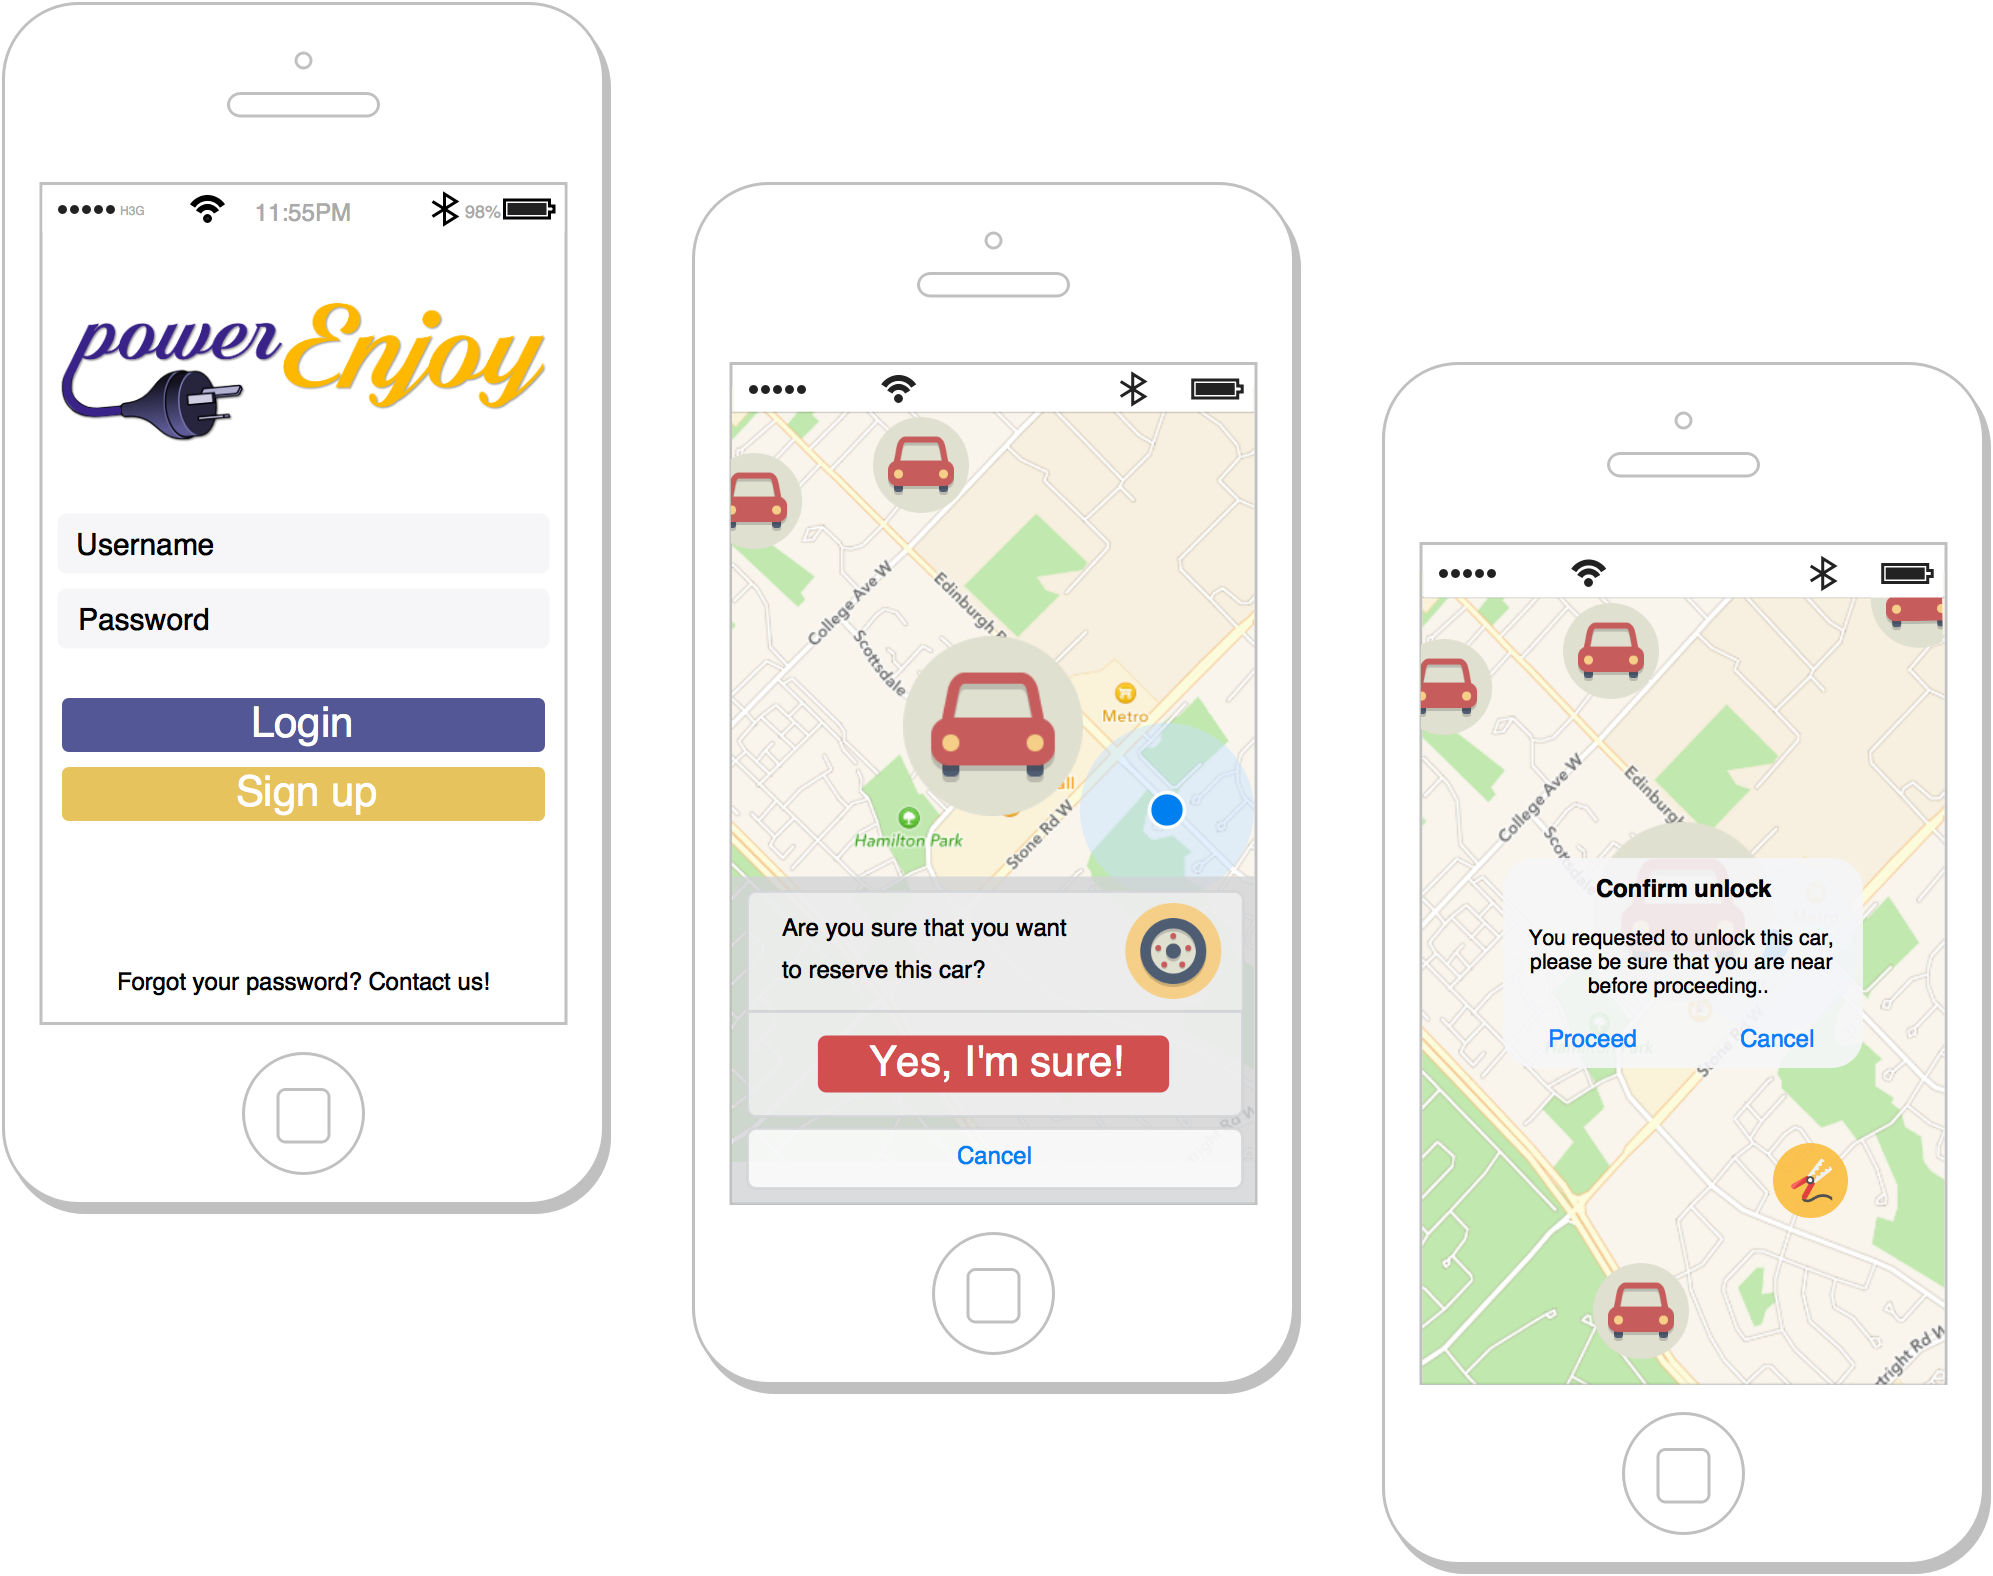
\includegraphics[width=1.0\textwidth]{/RASD/mobile_mockup}\\ 
	\vspace{0.5cm}
	\caption{3-page mockup representing the main pages of the mobile application} \label{fig:mobile_mockup} 
\end{figure}
Additional pages are the account management page, the payment page and maybe statistics related pages; those pages are not presented here as they are not strictly related to the application logic.

The web application will be really similar in features to the mobile application, the main use-cases are in fact the ones presented above in figure \ref{fig:mobile_mockup}; a basic mockup is presented (fig. \ref{fig:web_mockup}) to provide completeness:
\begin{figure}[!h]
	\centering
	\vspace{0.2cm}{}
	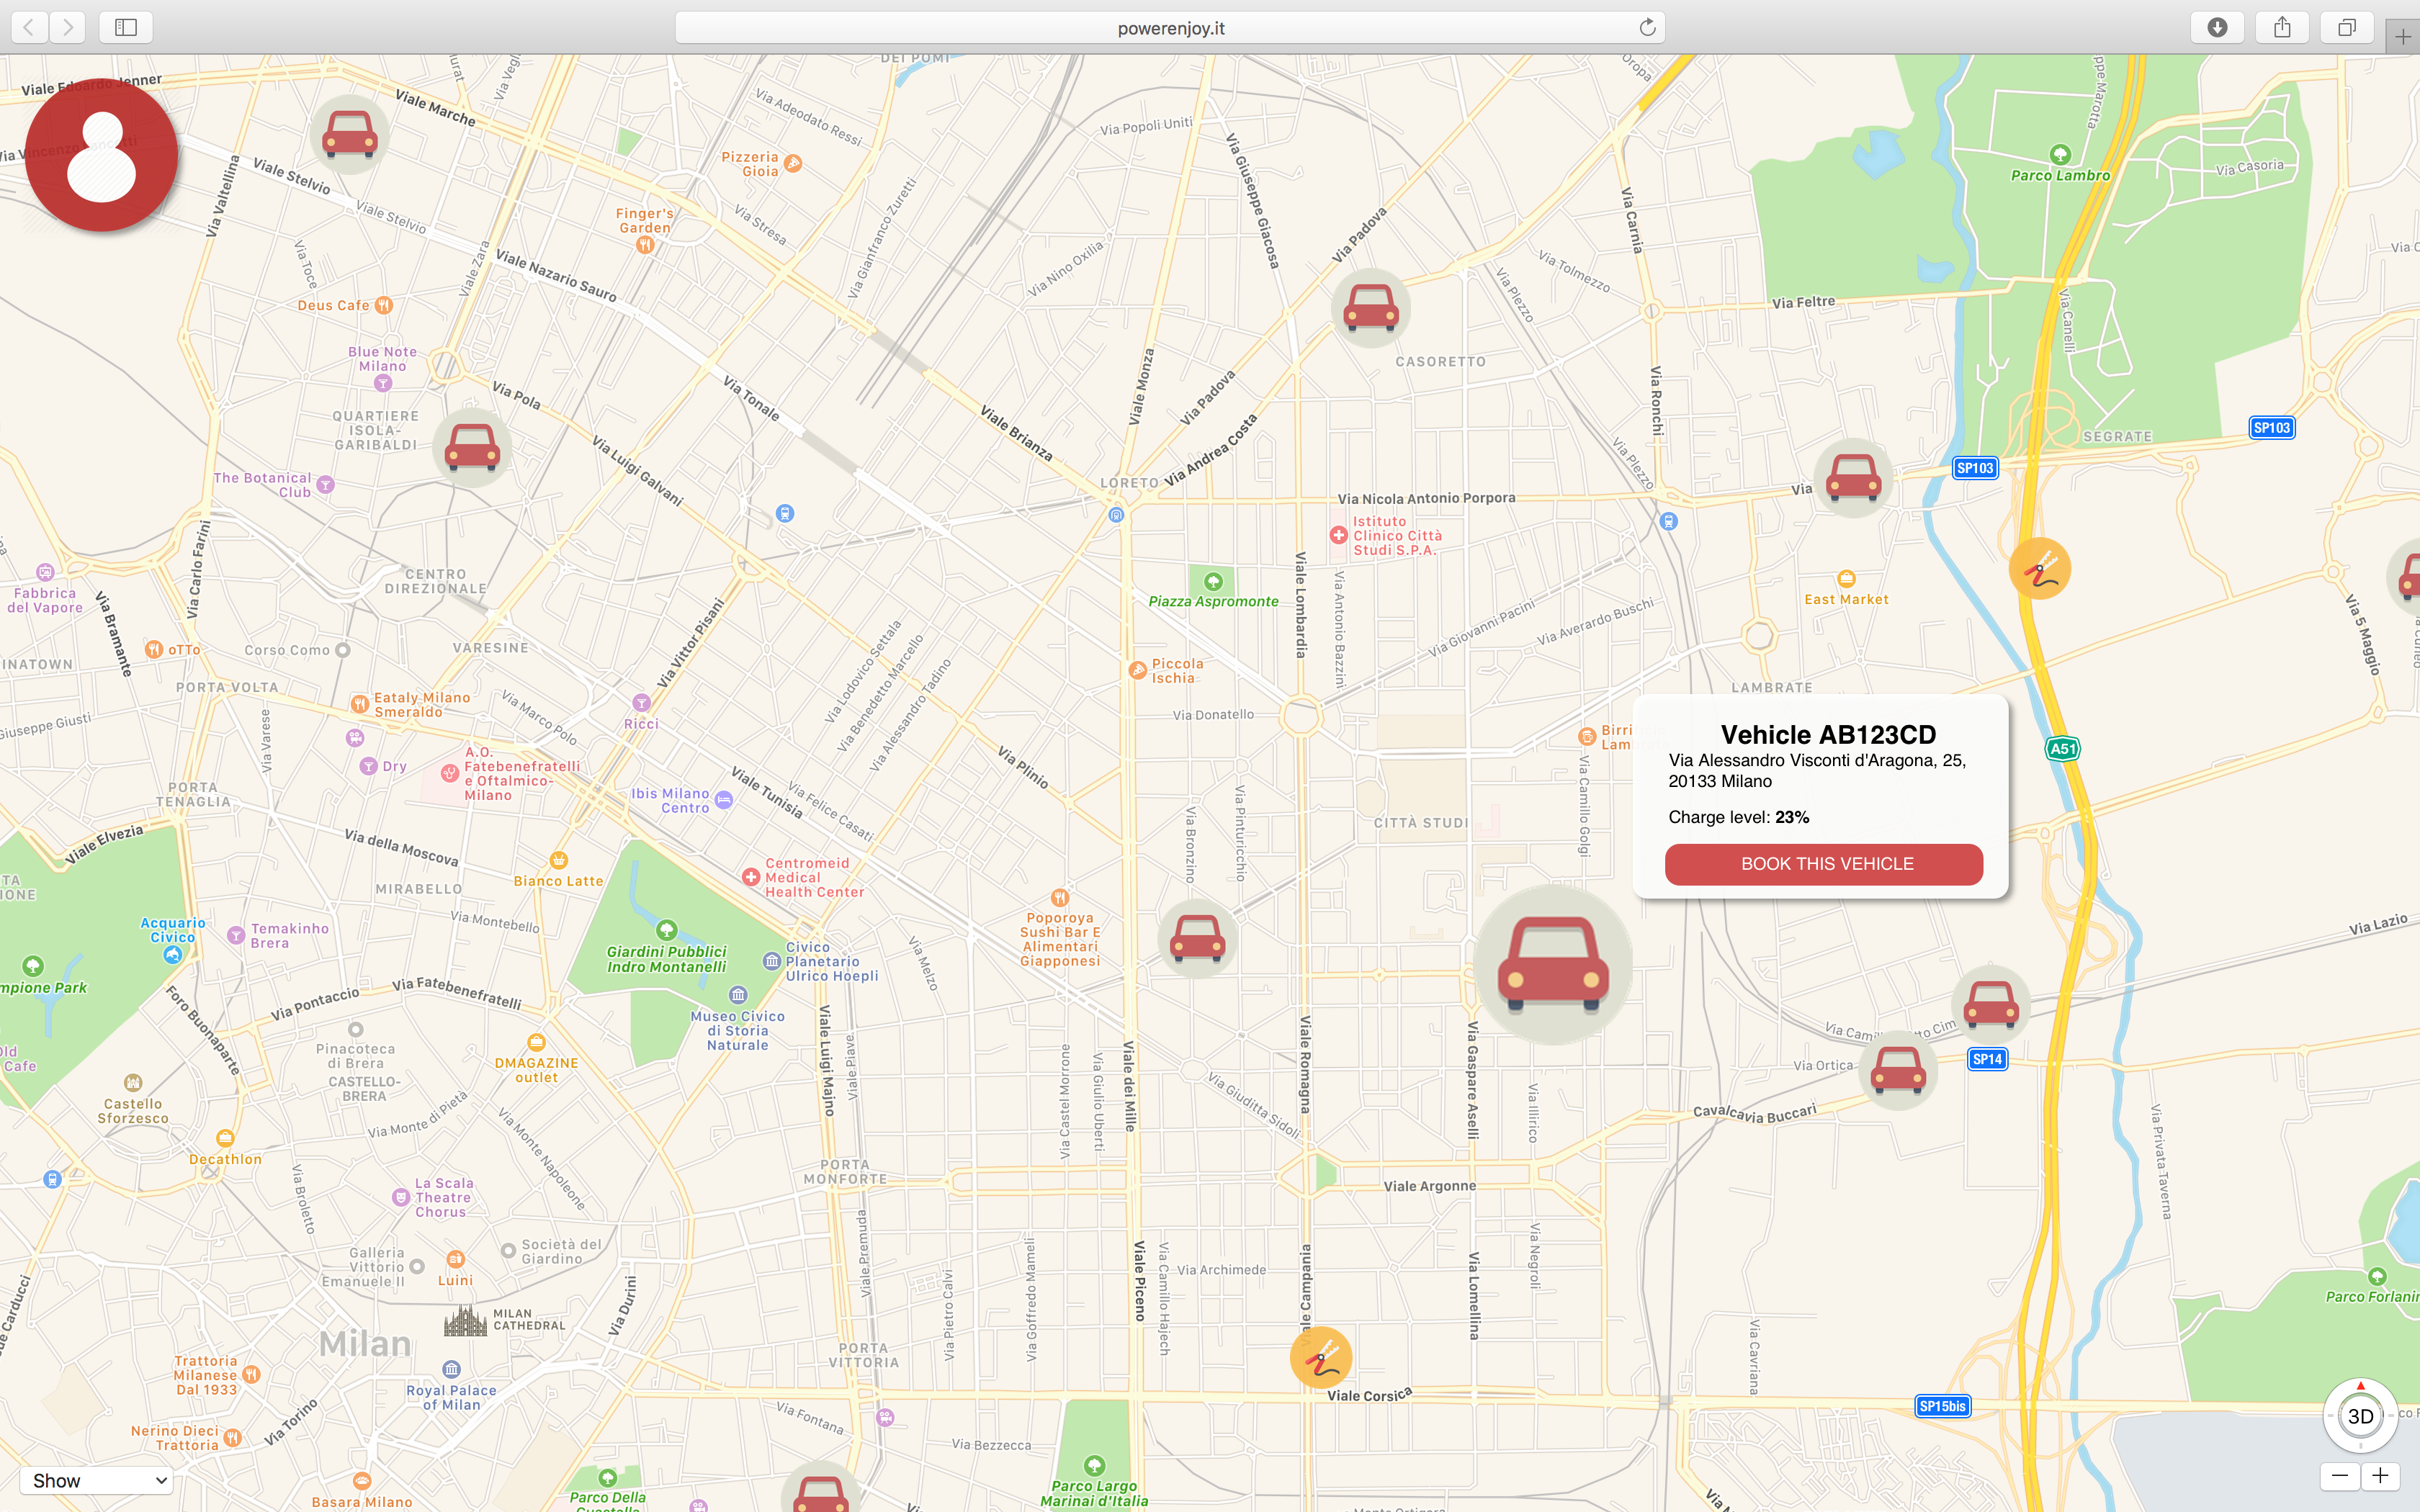
\includegraphics[width=1.0\textwidth]{/RASD/web_mockup}\\ 
	\vspace{0.5cm}
	\caption{1-page mockup representing the main page of the web application} \label{fig:web_mockup} 
\end{figure}
